\documentclass{article}
\usepackage[utf8]{inputenc}
\usepackage{graphicx}
\usepackage{amsmath}

\title{Homework Set 3 - PHYS 780 Solar Physics}
\author{Matthew Cooper}
\date{December 5th, 2018}
\begin{document}
\begin{titlepage}
\maketitle
\end{titlepage}

\textbf{Problem 5.1}:  A paper claims to detect spikes from a solar flare, based on the plot shown below.  Note the scale of solar flux units on the left, and the bar indicating the range corresponding to 1900 K in antenna temperature.  Show that these two scales are not consistent by calculating how many solar flux units would correspond to a 1900 K antenna temperature, given the following information: Trx = 2000 K, antenna diameter 1.5 m, zenith sky opacity t = 0.58, elevation angle 48 degrees, antenna efficiency h = 0.6.  What is the total atmospheric extinction at this elevation?  What is the total flux density corresponding to 1900 K before correction for atmospheric extinction?  After correction for extinction?  By what factor is the range of SFU in the figure too large?

\bigskip
\textbf{Solution}:  For this problem, we use the equation (4) from Lecture 5, 

\begin{equation}
T_{a} = \frac{S \eta A}{2k} 
\end{equation}

Solving in terms of S, and plugging in values of $T_a = 1900 K$, $A = \pi (.75)^2 m^2$ , $\eta = .6$, and $k = 1.38*10^{-22} m^2kgs^{-2}K^{-1}$, we get a value of $S = 494.58$ sfu before atmospheric extinction.  

For atmospheric extinction, we utilize equation (6) from Lecture 3 with a modification for the elevation angle, 

\begin{equation}
T_b = T_o e^{-\tau csc(E)} + T_e(1 - e^{-\tau csc(E)})
\end{equation}

Rearranging this equation for $T_o$, and plugging in values of $T_b = 1900 K$, $T_e = 300 K$, $\tau = .58$, and $E = 48^\circ$, we get a value of $T_o = 3791.98 K$, which corresponds to a flux density of $S = 963.13$ sfu.  Then the atmospheric extinction is given by 

\begin{equation}
\frac{\eta_{\nu}}{1 - \eta_{\nu}} = \frac{2k \nu^2T_{atmos}}{c^2}
\end{equation}

where $T_{atmos} = 300K$.  This yields $\eta_{\nu} = 8.26e-15$.The bar in the plot starts around 2.3 sfu, which is five times higher than the minimum should be.


\textbf{Problem 6.2}: Given two sources of amplitude a1 = 10 and a2 = 5, and spatial position q1 = 12 arcsec and q2 = -6 arcsec, what is the resultant amplitude and phase, ar and fr measured on a baseline of fringe spacing 54 arcsec?  If measured at 5 GHz, what projected baseline length between the two antennas does this fringe spacing correspond to?  What is the corresponding value of u, in wavelengths, assuming the baseline is entirely East-West?

\bigskip
\textbf{Solution}:  For the amplitude of the resultant wave, we utilize 
\begin{equation}
a_r = \sqrt{a_1^2 + 2a_1a_2 + a_2^2}
\end{equation}
which yields the result of $a_r = 15$.  Then, for the phase, we utilize
\begin{equation}
\phi_r = tan^{-1}\bigg(\frac{a_1 sin(\phi _1) + a_2 sin(\phi _2)}{a_1 sin(\phi _1) + a_2 sin(\phi _2)}\bigg)
\end{equation}
where $\phi _i = \frac{2\pi \theta _i}{\theta_{fringe}} $, which yields the result of $\phi _r = .705 $ rad.  For the projected baseline, use equation (2) from Lecture 6, which states 
\begin{equation}
\theta _{fringe} = \frac{c}{B_{proj}\nu}
\end{equation}
Solving this for $B_{proj}$ and inserting values $\theta _{fringe} = 54$ arcsec, $nu=5*10^9$ Hz, and the speed of light, we get $B_{proj} = 229.1$ m/rad, which converts to $u = 3818.3$ wavelengths.

\textbf{Problem 6.3}: Write a program (in IDL or MatLAB) to plot u,v coverage for the EOVSA array (latitude 37.23317 N), whose (E, N, U) antenna locations (in meters) are shown in the table below. Write the program to accept, as input parameters, the observing frequency, the source declination, and the hour angle range. Use your program to plot the u,v coverage for 10 GHz observing frequency, for (1) a source at declination d = $13^\circ$, and (2) a source at declination d = $0^\circ$. Both plots should cover an hour angle range -6h < h < +6h with 0.1 h resolution. In your plots, plot u on the horizontal axis, and v on the vertical axis, with (0,0) at the center of the plot, and use equal u and v scales ranging from -150 kl to 150 kl. Label the scales in kilowavelengths. Do not forget to plot both u,v points for a given baseline. Keep your program--you will be using a modified version of it in the following homework.

\bigskip
\textbf{Solution}:The solution program for this is included.  

\smallskip
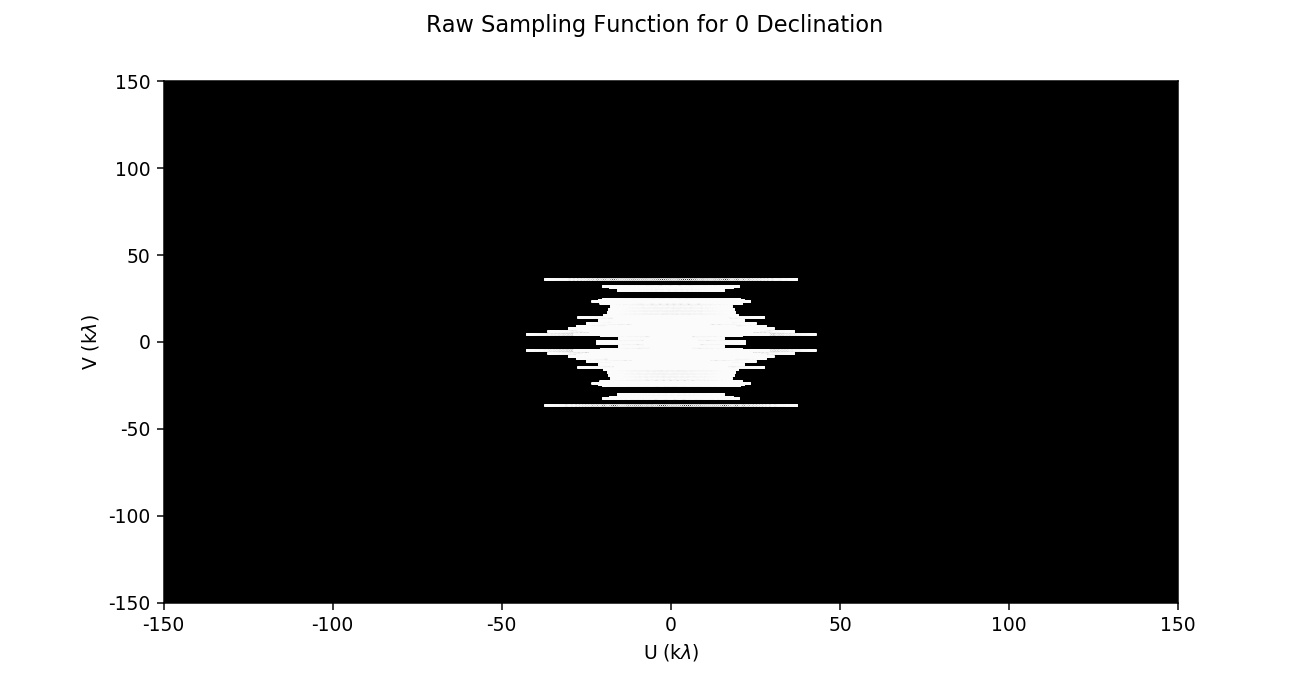
\includegraphics[scale=.5]{/media/mattcooper/64EC-62D6/RadioAstronomy/Homework6/UVPlotDec0.jpeg}

\smallskip
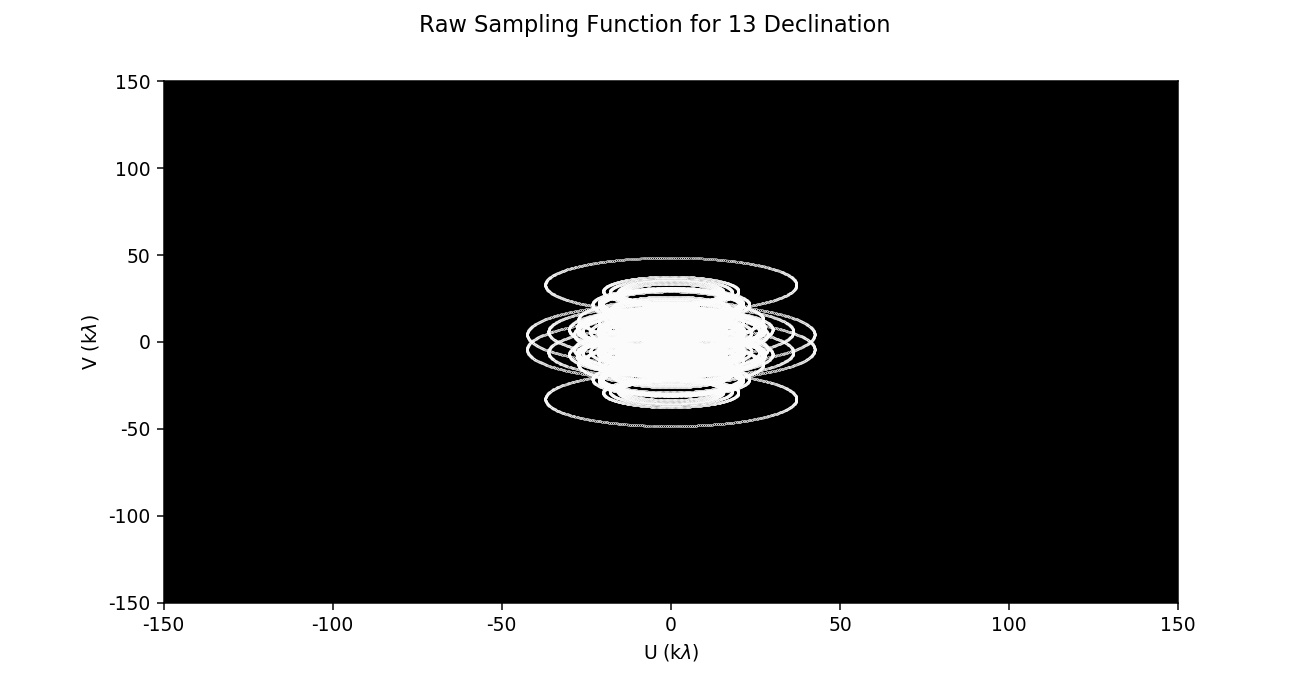
\includegraphics[scale=.5]{/media/mattcooper/64EC-62D6/RadioAstronomy/Homework6/UVPlotDec13.jpeg}

\textbf{Problem 6.4}:  In problem 6.3 of the previous homework, you wrote a program to calculate the u,v coordinates for 12 hours of observation with the EOVSA antennas. Now use them to obtain the synthesized beam (point spread function) of size 512 x 512 pixels by determining an appropriate scale Du, Dv for your u,v plane, gridding the u,v points to fall in the appropriate cell (pixel). Make two beams by following these two procedures: a) In each cell that has a u,v point, add the complex value complex(1,0). For cells that happen to have more than one u,v point (say n points in a cell), the value when you are done gridding will be complex(n,0). This is called "natural weighting." Then do an FFT, and make a print-out of the inner 128x128 cells of the synthesized beam (after shifting by 256,256) as a contour map with contours ranging from -50\% to +100\% of the peak value (which should be in the center, after shifting). Draw the +50\% contour using a different color, or with a thicker line, to make it stand out. b) Do the same procedure, but now using "uniform weighting" where each cell with u,v points in it has a value complex(1,0), no matter how many u,v points may fall into it. Submit your calculation of the Du, Dv scale, the corresponding Dq angular scale of the beam (arcmin/cell), your code, and the two contour plots with x,y axes labeled in arcmin. Measure somehow the major and minor axis of the 50\% contour and write down the sizes (full-width-half-maximum) in arcsec. Which one has the best resolution (smallest beam), uniform or natural weighting?

\bigskip
\textbf{Solution}:  The scales for Du and Dv can be found by dividing the original scale length (300000 wavelengths) by the number of pixels, which yields Du = Dv = 585.9375 wavelengths per pixel. The angular width is the determined using 
\begin{equation}
\triangle \ theta = (N\triangle s)^{-1}
\end{equation}

Plugging in N = 512 and $\triangle s = 585.9375$, we get an angular scale of $\triangle \theta = 3.33$ $\mu rad$.

\smallskip
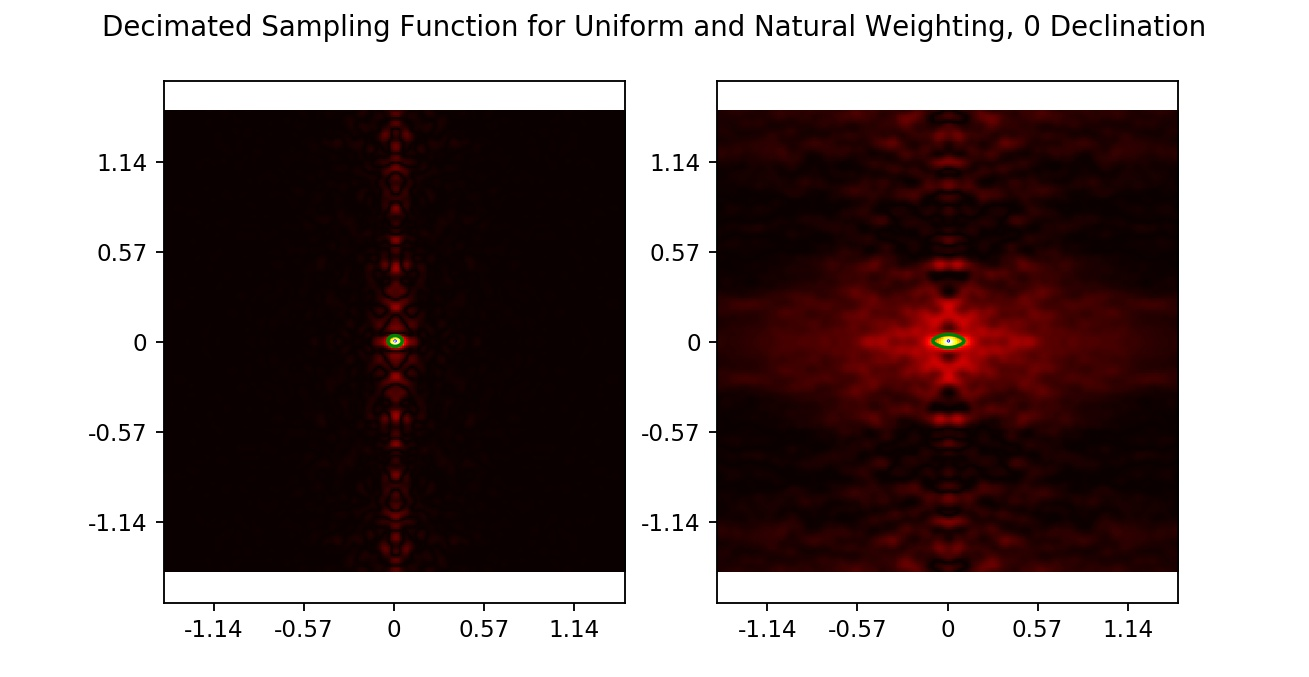
\includegraphics[scale=.5]{/media/mattcooper/64EC-62D6/RadioAstronomy/Homework6/Decimated0Decl.jpeg}

\smallskip
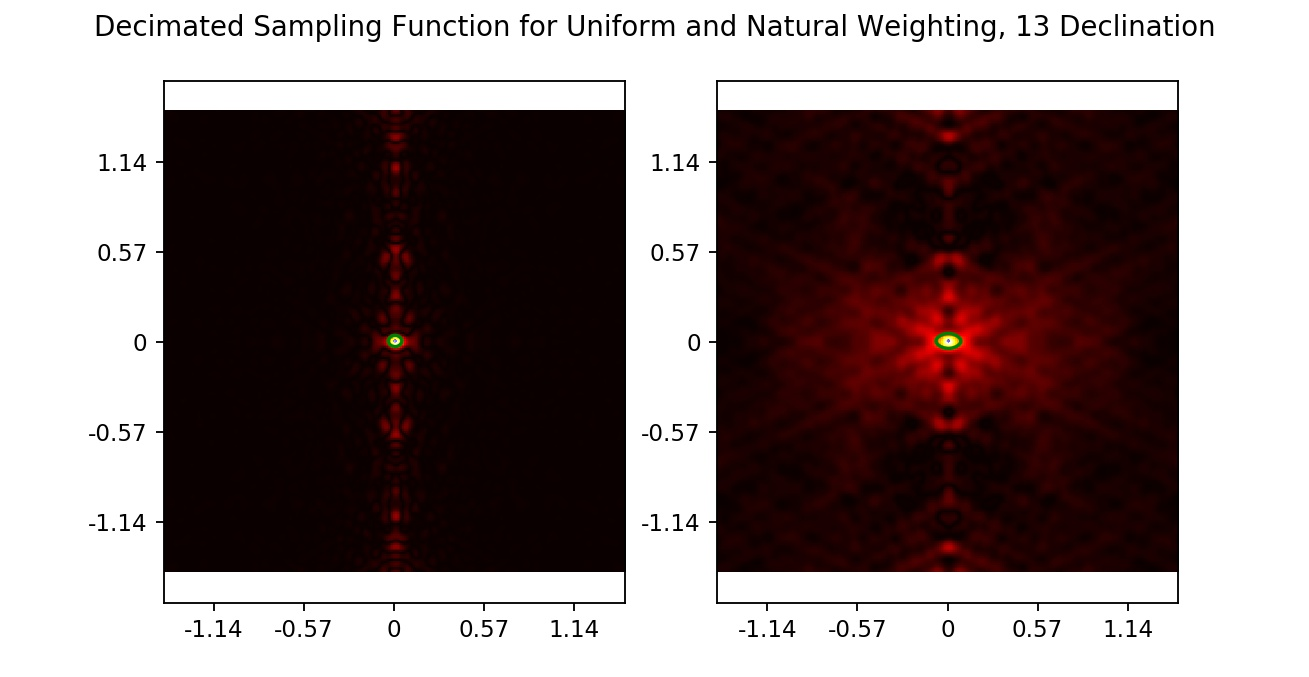
\includegraphics[scale=.5]{/media/mattcooper/64EC-62D6/RadioAstronomy/Homework6/Decimated13Decl.jpeg}

The beam width for the uniform sampling at is around 76 arcsec for the major axis, and 68 arcsec for the minor axis. The natural sampling is about 182.4 arcsec for the major axis and 84.4 arcsec for the minor.

The uniform weighting will yield the best resolution, since the power is more tightly concentrated.

\textbf{Problem 6.5}:  Download the file uvmodel.sav (IDL) or uvmodel.mat (MATLAB), which is the fourier transform of a model sky brightness distribution, and apply your two (uniform and natural weighted) gridded u,v point arrays as a sampling function, then do the inverse FFT on the sampled data to obtain dirty maps for the two cases. (a) Display the two images side-by-side, with appropriate annotation, and turn in your code and the images. Note, the zero for the uv data and for the images is the bottom left corner, so to display these items with the zero in the center you will have to shift by 256 pixels in each dimension first. (b) For the natural weighting case, make a six-panel figure like that of Fig. 10 in lecture 6. Label the panels appropriately. Turn in your code for this 6-panel figure as well.

\bigskip
\textbf{Solution}:

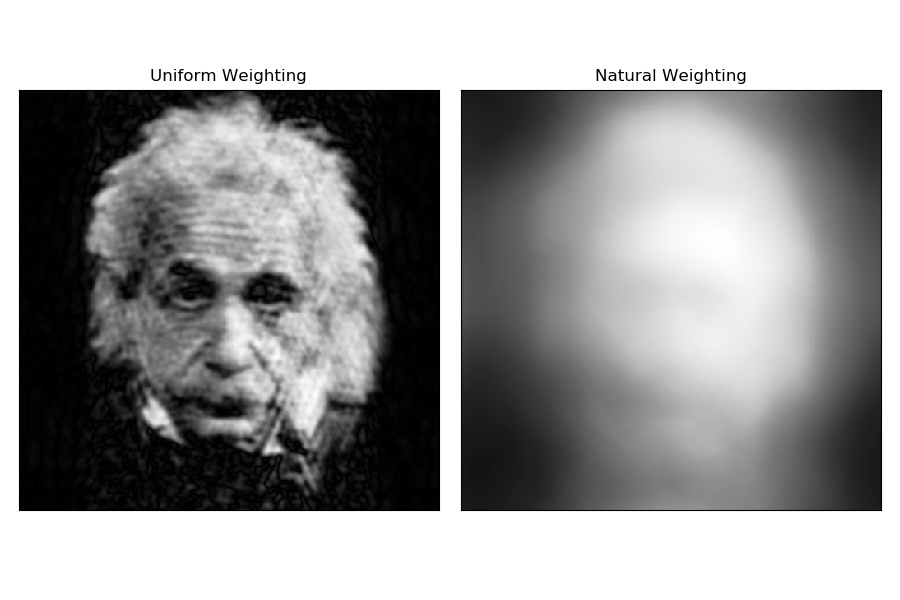
\includegraphics[scale=.5]{/media/mattcooper/64EC-62D6/RadioAstronomy/Homework6/UniNat.jpeg}

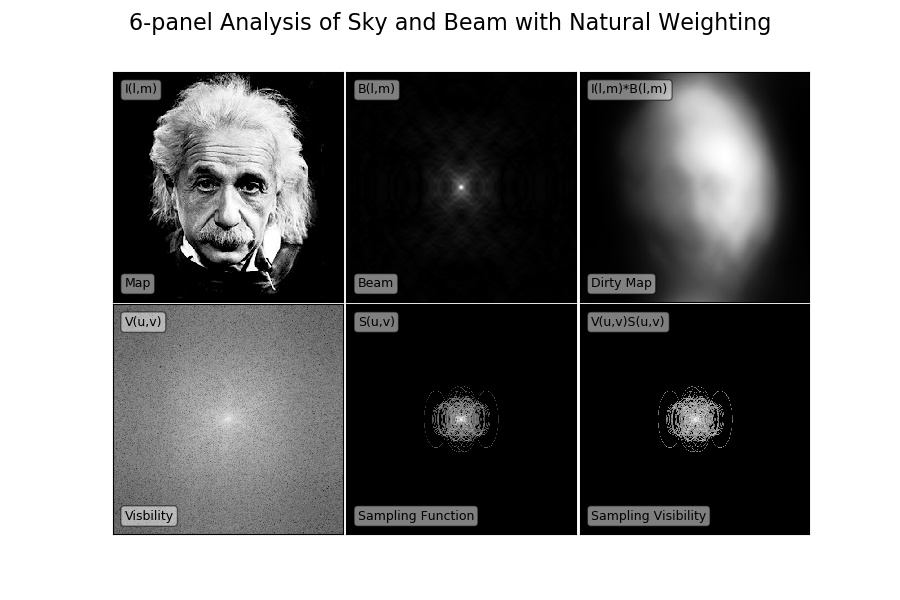
\includegraphics[scale=.5]{/media/mattcooper/64EC-62D6/RadioAstronomy/Homework6/6PanelNat.jpeg}





\end{document}